\documentclass[letter]{article}
\usepackage{amsmath}
\usepackage{amsfonts}
\usepackage{amssymb}
\usepackage{ifthen}
\usepackage{fancyhdr}
\usepackage{graphicx}
\usepackage{subcaption}
\usepackage[shortlabels]{enumitem}

%%%
% Set up the margins to use a fairly large area of the page
%%%
\oddsidemargin=.2in
\evensidemargin=.2in
\textwidth=6in
\topmargin=0in
\textheight=9.0in
\parskip=.07in
\parindent=0in
\pagestyle{fancy}

%%%
% Set up the header
%%%
\newcommand{\setheader}[6]{
	\lhead{{\sc #1} {\sc #2}\\{} ({\small \it \today})}
	\rhead{
		{\bf #3} 
		\ifthenelse{\equal{#4}{}}{}{(#4)}\\
		{\bf #5} 
		\ifthenelse{\equal{#6}{}}{}{(#6)}%
	}
}

\begin{document}
	\setheader{CSC490}{Module 1}{Qiwen Hua}{}{Ben Weisz}{}
	
	\setcounter{section}{2}
	\subsection{LiDAR Voxelization}

	\textbf{Part 2:} In the implementation of the \verb|Voxelizer.forward| function, we map raw LiDAR points to voxels by taking the difference between the points and bounds (e.g. \verb|x_max|) and scale down by `step`. Therefore, larger \verb|step| yields lower resolution for the voxelized point clouds, thus decreases the amount of captured information. 

	We can visualize the conclusion above by plotting the voxelized LiDAR point clouds for scene \verb|000| with four different \verb|step|s $\in \{0.25, 0.50, 1.00, 2.00\}$. The plots are shown below:

	\begin{figure}[h]
		\begin{subfigure}[t]{\textwidth}
			\centering
			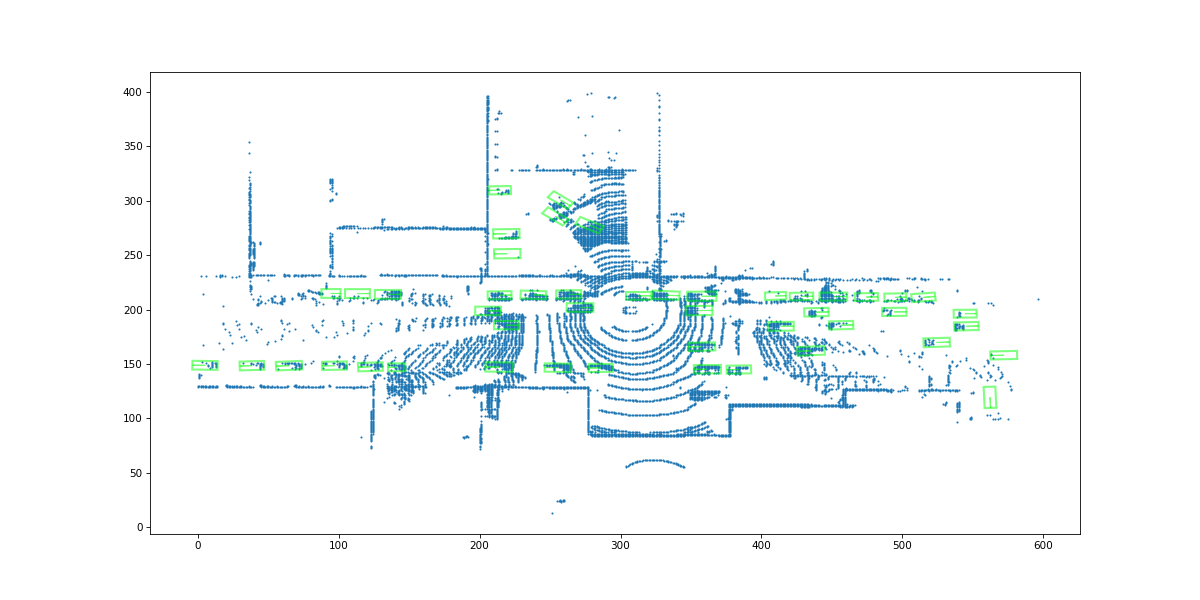
\includegraphics[width=\linewidth]{images/vox000_step0-25.png}
			\vspace*{-10mm}
			\caption{step = 0.25}
		\end{subfigure}
	  
		\begin{subfigure}[t]{\textwidth}
			\centering
			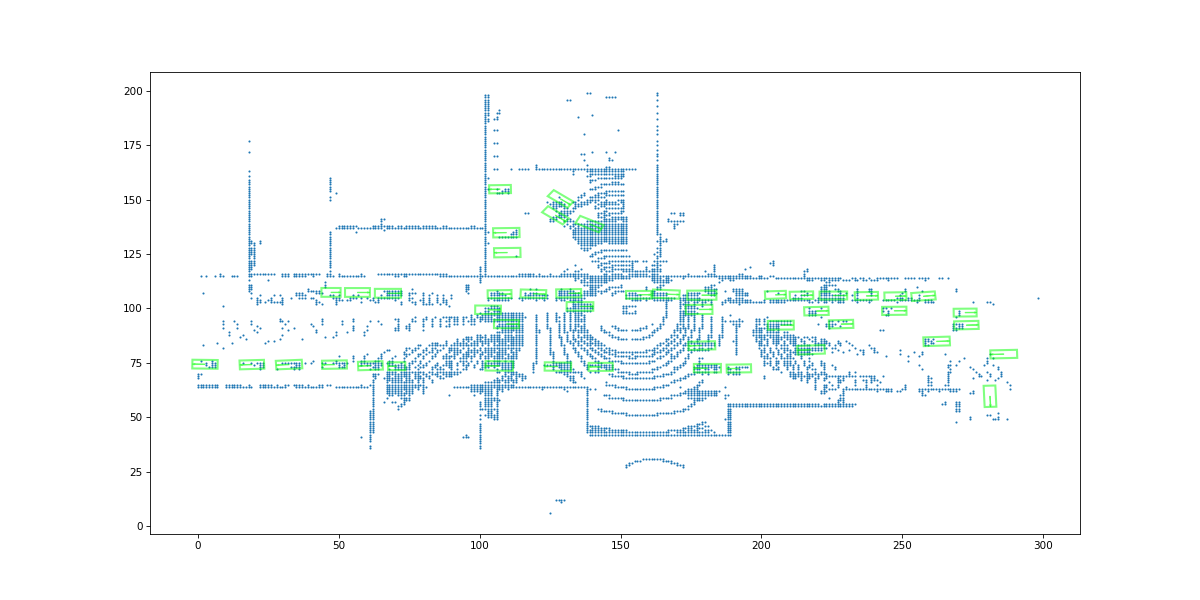
\includegraphics[width=\linewidth]{images/vox000_step0-50.png}
			\vspace*{-10mm}
			\caption{step = 0.50}
		\end{subfigure}
	\end{figure}

	\begin{figure}[h]
		\begin{subfigure}[t]{\textwidth}
			\centering
			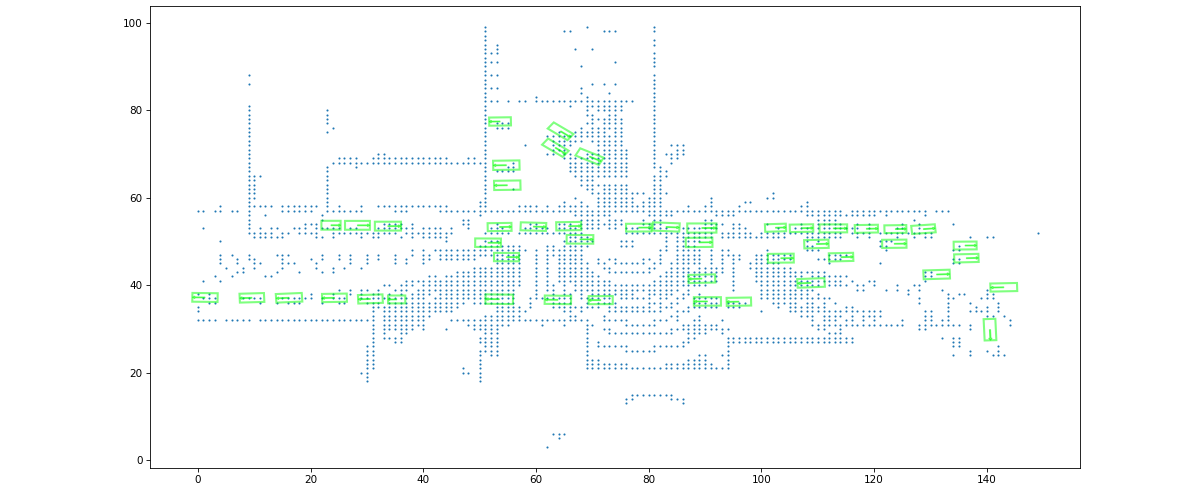
\includegraphics[width=\linewidth]{images/vox000_step1-00.png}
			\vspace*{-10mm}
			\caption{step = 1.00}
		\end{subfigure}
	  
		\begin{subfigure}[t]{\textwidth}
			\centering
			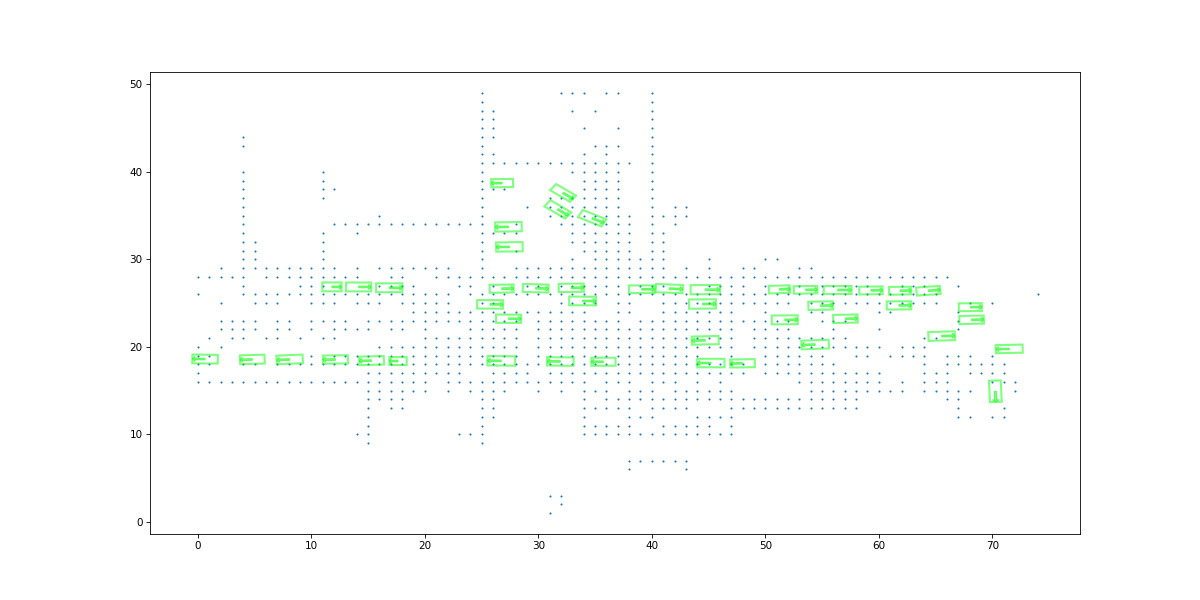
\includegraphics[width=\linewidth]{images/vox000_step2-00.png}
			\vspace*{-10mm}
			\caption{step = 2.00}
		\end{subfigure}
	\end{figure}

	From the plots above and below, we can see that the image with the highest resolution (a) captures much more information than the image with the lowest resolution (d). However, in order to have high fidelity of the voxel grid, the grid size also needs to be larger. Namely, image (a) has a size of 600 by 400 while image (d) has a size of 75 by 50; the size of the former grid is 64 times larger than the latter. 

	Therefore, we can conclude that the fidelity of the voxel grid comes at the cost of larger memory consumption (to store the larger grid). In addition, performance is also sacrificed as more captured information (voxel points) leads to more intensive computations. 

\end{document}
